\documentclass[bosnian,12pt,a4paper]{report}
\usepackage[utf8]{inputenc}
\usepackage[T1]{fontenc}
\usepackage{mathpazo}
\usepackage[autostyle=true]{csquotes}
\usepackage[document]{ragged2e}
\usepackage{amsfonts,amsmath,amssymb}
\usepackage{amsmath,multicol,eso-pic}
\usepackage[utf8]{inputenc}
\usepackage[T1]{fontenc}
\usepackage[]{geometry}
\usepackage{babel}
\usepackage{enumerate}
\usepackage{titlesec}
\usepackage{breqn}
\usepackage{tikz}
\usepackage{rotating}
\usepackage{tikz}
\usetikzlibrary{automata, positioning}
\usepackage[makeroom]{cancel}
\usepackage{textcomp}
\usepackage{mathtools}
\usepackage{multirow}
\usepackage{hyperref}
\usepackage{secdot}
\usepackage{tocloft}
\renewcommand{\contentsname}{Sadržaj}
%\usepackage{lipsum}
\titlespacing*{\chapter}{0pt}{-20pt}{40pt}
\titleformat{\chapter}[display]
{\huge\bfseries\centering}
{}
{0pt}
{\thechapter.\ }
\titleformat{name=\chapter,numberless}[display]
{\huge\bfseries}
{}
{0pt}
{}
\def\frontmatter{%
    \pagenumbering{roman}
    \setcounter{page}{1}
	\renewcommand{\thesection}{\Roman{section}}
}%
\def\mainmatter{%
	\pagenumbering{arabic}
	\setcounter{page}{1}
	\setcounter{section}{1}
	\renewcommand{\thesection}{\arabic{chapter}.\arabic{section}}
}%

\geometry{
	paper=a4paper,
	inner=2.5cm,
	outer=2.5cm,
	bindingoffset=.5cm,
	top=1.5cm,
	bottom=1.5cm,
}

\hypersetup{pdfpagemode={UseOutlines},
	bookmarksopen=true,
	bookmarksopenlevel=0,
	colorlinks=true,
	citecolor=magenta,
	linkcolor=red!30!black,
	urlcolor=red!50!black,
	pdfstartview={FitV},
	unicode,
	breaklinks=true,
}

\renewcommand{\cftchapleader}{\cftdotfill{\cftdotsep}}
\renewcommand{\cftsecleader}{\cftdotfill{\cftdotsep}}

\setcounter{secnumdepth}{3}
\setcounter{tocdepth}{2}



\begin{document}
	\frontmatter
	\pagestyle{plain}
	
	\begin{titlepage}
	
	
		\begin{center}
		\textsc{\huge Seminarski rad}\\[0.3cm] 
		\textsc{\Large iz predmeta}\\[0.3cm] 
		\textsc{\huge Numerički algoritmi} \\
		\vspace{1.5cm}
		
		\hrulefill \\[0.2cm]
		{\huge \bfseries Newton-ov metod za minimizaciju funkcija više nezavisnih promjenljivih, uz razne varijante izbora koraka duž odabranih pravca \par}\vspace{0.2cm}
		\hrulefill \\[2cm]
		
		
		\begin{minipage}[t]{\textwidth}
			\begin{flushleft} \large
				\emph{Autori:}\\[0.1cm]
				{Anel \textsc{Mandal} \\
				 Lejla \textsc{Mehmedagić}}
			\end{flushleft}
		\end{minipage}
		\begin{minipage}[t]{\textwidth}	
			\begin{flushright} \large
				\emph{Profesor:} \\
				{prof. dr. Željko \textsc{Jurić}, dipl.ing.el.}  
			\end{flushright}
		\end{minipage}\\[0.5cm]
		\begin{minipage}[t]{\textwidth}	
			\begin{flushright} \large
				\emph{Asistent:} \\
				{Šeila \textsc{Bečirović}, BA ing.}  
			\end{flushright}
		\end{minipage}\\[3cm]
		
		
		{\scshape\LARGE \href{http://etf.unsa.ba/}{Elektrotehnički fakultet}\par}\vspace{0.25cm}
		{\scshape\LARGE \href{https://en.wikipedia.org/wiki/Sarajevo}{Sarajevo} \par}\vspace{4cm}
		\vfill
		
		{\large \today}
		\vfill
		\end{center}
	\end{titlepage}

\clearpage
\newpage
\begin{abstract}
\justify
U ovom radu prezentirati ćemo jednu od više metoda za višedimenzionalnu minimizaciju, tačnije Newton-ov metod koji pripada skupini metoda pretraživanja po pravcu. Kod ovih metoda se, polazeći od neke tačke bira neki pravac nakon čega se traži minimum duž tog pravca. Osvrnut ćemo se na klasični Newton-ov metod a finalna implementacija prezentirati će također kvazi-Newton metod koji predstavlja značajno poboljšanje klasičnog, s obzirom da isti nije primjenjiv u praksi. Cilj je dakle ostvariti nešto bržu a i precizniju aproksimaciju u odnosu na klasični metod. Poglavlje "Uvod" sadrži opis algoritma te probleme koje je potrebno riješiti prilikom konstrukcije istog. "Implementacija algoritma" sadrži sam pseudokod, koji će u ovom radu biti direktno implementiran u paketu numeričkog računanja Scilab. Rad završavamo sa nekim testiranjem u cilju utvrđivanja efikasnosti i preciznosti samog algoritma te se kratko osvrćemo i na samo primjene istog.\\

\vspace*{0.5cm}

\begin{center}
\textbf{Abstract}
\end{center}

\justify
In this paper, we will present one of several methods for multi-dimensional minimization, specifically Newton's method, which belongs to a group of line search methods. In these methods, we start from a specific point, choose a direction, which we move along to find a minimum. We will discuss the classic Newton method, and the final implementation will also present a quasi-Newton method that represents a significant improvement of the classic one, since it is not applicable in practice. Therefore,  the goal is to achieve a faster and more precise approximation. Chapter "Uvod" contains a description of the algorithm and problems that need to be solved when constructing it. "Implementacija algoritma" contains the pseudocode itself, which in this paper will be directly implemented in the Scilab numerical computational package. We end the paper with some tests in order to determine the efficiency and precision of the algorithm itself, we also briefly look at its applications.


\end{abstract}

\clearpage
\newpage
\tableofcontents

\newpage
\mainmatter
\chapter{Uvod}
	\section{Minimizacija metodom pretraživanja po pravcu}
	
	\justify
	Optimizacioni algoritmi su iterativni. Dakle, započinje se sa nekom početnom pretpostavkom varijable $x$ te se generiše sekvenca poboljšanjih pretpostavki, dok se ista ne terminira, nadajmo se u rješenju. Kod metoda pretraživanja po pravcu se, polazeći od neke tačke $\textbf{x}^*$ bira neki pravac, odnosno vektor $\textbf{p}$, nakon čega se traži minimum duž tog pravca. 
	\justify
	Tačke duž tog pravca imaju oblik $x^* + h\textbf{p}$ s obzirom da taj pravac prolazi kroz tačku $x^*$ a određen je vektorom $\textbf{p}$ gdje h predstavlja predstavlja dužinu koraka duž odabranog pravca ($h \in \mathbb{R}$). 
	
	
	\justify
	Ciljna funkcija $f$ je, duž odabranog pravca, funkcija samo jedne realne promjenljive $h$, koju ćemo označiti sa $\varphi(h) = f(\textbf{x}^* + h\textbf{p})$. Iz ovoga neposredno slijedi da se za minimizaciju funkcije $\varphi(h)$ mogu koristiti neke od tehnika za nalaženje minimuma funkcije jedne realne promjenljive, kao što je recimo Brentov\footnote{Richard Peirce Brent (1946-), australijski matematičar i informatičar} algoritam. 
	
	\justify
	Nakon pronalaska koraka $h^*$ koji minimizira funkciju $\varphi$, tačka $\textbf{x}^* + h\textbf{p}$ se uzima za novu tačku, nakon čega se bira novi pravac te se postupak ponavlja dok se ne utvrdi da se nalazimo u minimumu, ili barem njegovoj okolini, što sve zavisi od same implementacije algoritma.
	
	
	\justify
	Prirodno se postavlja pitanje određivanja koraka $h$. Strategija kod koje se korak $h$ bira tako da se minimizira funkcija $\varphi(h)$, kao što je to navedeno iznad, naziva se \textit{egzaktno pretraživanje po pravcima}. 
	
	
	\justify
	Međutim, ova strategija se ne primjenjuje u praksi s obzirom da nalaženje minimuma funkcije $\varphi(h)$ samo za sebe može biti dosta zahtjevno. Stoga se javlja potreba za drugačijom strategijom, kao što je recimo \textit{neegzaktno pretraživanje po pravcima} kod koje se zadovoljavamo sa tačkom u kojoj je funkcija \textit{dovoljno opala} u odnosu na trenutnu tačku. 
	
	
	
	\justify
	Ipak, potrebno je i dalje postaviti određene uvjete na korak jer se može desiti da se konvergencija ne postigne prilikom lošeg izbora. S tim na umu, postoji nekoliko uvjeta, koji mogu garantirati validan izbor koraka $h$ a koje ćemo diskutovati dalje u nastavku. 
	
	
	\justify
	Međutim, izbor koraka nije najveći problem ovih metoda već izbor pravca. Većina metoda bira silazne pravce, odnosno pravce duž kojih ciljna funkcija opada od polazne tačke. S obzirom da se ovaj rad bavi Newtonovim\footnote{Isaac Newton (1642 – 1717), engleski fizičar, matematičar i astronom} metodama za minimizaciju nećemo se upuštati u mnogobrojne načina izbora pravca. Neki od metoda, kao što je upravo i Newtonov, u svakoj iteraciji predlažu ne samo pravac nego čak i korak. Treba naglasiti da nemamo garanciju da je taj pravac odnosno korak ujedno i validan. O ovome ćemo također diskutovati u nastavku.
	
	\section{Newton-ov metod}
	Razmotrimo problem minimizacije bez ograničenja
	\\
	$$min~f(x)$$
	$$x \in \mathbb{R}^n, ~n=1$$
	
	Neka je $f : R \rightarrow R$ dva puta diferencijabilna funkcija. Tada
	se ista može razviti u Taylorov\footnote{Brook Taylor (1685–1731) je bio engleski matematičar, najbolje poznat po Taylorovom teoremu i Taylorovom redu} polinom drugog stepena u okolini trenutne aproksimacije $x^*$ kao
	
	\vspace{0.25cm}
	$$f(x) \approx f(x^* + (x - x^*)) \approx f(x^*) + f'(x^*)(x-x^*) + \frac{1}{2}f''(x^*)(x-x^*)^2, ~~ k \in \mathbb{N}$$
	
	\vspace{0.5cm}
	Nova iteracija može se izračnati kao tačka u kojoj izvod aproksimativne funkcije ima vrijednost 0, pri čemu se dobija
	\vspace{0.5cm}
	
	$$0 = f'(x^*) + f''(x^*)(x-x^*)$$
	
	\vspace{0.5cm}
	odnosno, imamo Newton-ov iterativni proces
	\vspace{0.5cm}
	
	$$x_{i} = x^*_{x-1} - \frac{f'(x^*_{x-1})}{f''(x^*_{x-1})}, ~~ i \in \mathbb{N}$$
	
	\vspace{1cm}
	Lahko se primijeti da ovo nije ništa drugo nego Newtonov metod za rješavanje nelinarne jednačine $f'(x)=0$. S tim na umu možemo zaključiti da ovaj metod ima kvadratnu konvergenciju. \\ S obzirom da nas zanimaju funkcije više nezavisnih promjenljivih nećemo se upuštati u algoritam za ovaj specijalan slučaj, odnosno kada je $n=1$.
	
	\vspace{1.5cm}
	Razmotrimo, dakle, generalniji slučaj, odnosno
	
	$$min~f(x)$$
	$$x \in \mathbb{R}^n, ~~ n \geq 2$$
	
	\vspace{0.5cm}
	Oko tačke $x^{*}$ (početna aproksimacija minimuma), funkcija $f$ se može aproksimirati sa Taylorovim polinomom drugog reda na sljedeći način:
	
	$$f(x) \approx f(\textbf{x}^* + (\textbf{x} - \textbf{x}^*)) \approx f(\textbf{x}^* + h\textbf{p}) \approx f(\textbf{x}^*) + \triangledown f(\textbf{x}^*)^T h\textbf{p} + \frac{1}{2} h \textbf{p}^T \triangledown^2 f(\textbf{x}^*) h \textbf{p}$$
	
	Ako uzmemo $h\textbf{p} = \textbf{t}  = \textbf{x}-\textbf{x}^*$ 
	
	$$f(\textbf{x} + \textbf{t}) = q(\textbf{t}) = f(\textbf{x}^* + (\textbf{x} - \textbf{x}^*)) = f(\textbf{x}^*) + \triangledown f(\textbf{x}^*)^T \cdot\textbf{t} + \frac{1}{2} \textbf{t}^T \triangledown^2 f(\textbf{x}^*)\textbf{t}$$
	
	\newpage
	Pri čemu vrijedi sljedeće:
	
	\begin{itemize}
		\item $h \in \mathbb{R}$, je korak duž odabranog pravca
		\item $\textbf{p} \in \mathbb{R}^n$, je pravac (odnosno vektor) duž kojeg tražimo minimum
		\item $\triangledown f(\textbf{x}^*)$ - gradijent funkcije u tački $\textbf{x}^*$
		\item $\triangledown^2 f(\textbf{x}^*)$ - Hessian funkcije u tački $\textbf{x}^*$
	\end{itemize}
	
	\vspace{0.5cm}
	
	\justify
	Narednu aproksimaciju minimuma funkcije $f$ ćemo aproksimirati sa minimumom model funkcije $q(\textbf{t})$. Navesti ćemo prvo nekoliko teorema diferencijalnog računa koji će nam poslužiti za nalaženje izvoda ove model funkcije. Potrebno je dakle naći izvod po $\textbf{t}$. \\Napomenimo da, ukoliko su $\frac{\partial^2 f}{\partial x_1 \partial x_j}$ neprekidni u okoličini tačke $\textbf{a}$, \\ za $\forall i,j = 1,...,n$, vrijedi da je Hessian simetrična matrica.
	
	
	\vspace{1cm}
	\hrulefill \\[0.4cm]
	\textbf{\textit{Teorema 1}}: Neka je $\textbf{a} \in R^n$ konstantan vektor i neka je funkcija  $\textbf{f} : R^n \rightarrow R$ definisana kao:
	
	$$\textbf{f}(\textbf{x}) = \textbf{a}, ~ \textbf{x} \in R^n$$
	
	Tada važi:
	
	$$\frac{d\textbf{f}(\textbf{x})}{d\textbf{x}} = \textbf{0}, \in R^n$$
	
	\hrulefill \\
	\vspace{0.4cm}
	\textbf{\textit{Teorema 2}}: Neka je $\textbf{a} \in R^n$ konstantan vektor i neka je funkcija  $\textbf{f} : R^n \rightarrow R$ definisana kao:
	
	$$\textbf{f}(\textbf{x}) = \textbf{a}^T \textbf{x}, ~ \textbf{x} \in R^n$$
	
	Tada važi:
	
	$$\frac{d\textbf{f}(\textbf{x})}{d\textbf{x}} = \textbf{a}, \textbf{x} \in R^n$$
	
	\vspace{1cm}
	\hrulefill \\
	
	\vspace{1cm}
	U teoriji optimizacije vrlo bitnu ulogu imaju simetrične matrice, tj. primjenjivat ćemo sljedeću teoremu 
	
	\newpage
	\hrulefill \\ 
	\textbf{\textit{Teorema 3}}: Neka je $\textbf{A} \in R^n$ simetrična matrica i neka je funkcija  $\textbf{f }: R^n \rightarrow R$ definisana kao:
	
	$$\textbf{f}(\textbf{x}) = \textbf{x}^T A\textbf{x}, ~ \textbf{x} \in R^n$$
	
	Tada važi:
	
	$$\frac{d\textbf{f}(\textbf{x})}{d\textbf{x}} = 2A\textbf{x}, \textbf{x} \in R^n$$
	
	\hrulefill \\
	
	\vspace{1cm}
	Imajući ove teoreme na umu lahko se nalazi izvod model funkcije koji glasi:
	
	$$\triangledown q(\textbf{t}) = \triangledown f(x^*) + \triangledown^2 f(x^*) \cdot \textbf{t}$$
	
	\vspace{1cm}
	Prepostavimo sada da je nova tačka  $ \textbf{t} = \textbf{x}^* + h\textbf{p}$ upravo tražena tačka minimuma. U toj tački mora vrijediti $\triangledown f(\textbf{x}^* + h\textbf{p}) = 0$, onda imamo 
	
	\vspace{0.2cm}
	$$0 \approx \triangledown f(x^*) + \triangledown^2 f(x^*) \cdot h\textbf{p}$$
	
	\vspace{0.3cm}
	Sada, uz pretpostavku da je Hessian simetrična matrica, imamo
	
	\vspace{0.3cm}
	$$h\textbf{p} \approx -\triangledown ^2 f(\textbf{x}^*)^{-1} \triangledown f(\textbf{x}^*)$$
	
	\vspace{0.3cm}
	odnosno, koristeći matrično lijevo dijeljenje,
	
	\vspace{0.3cm}
	$$h\textbf{p} \approx -\triangledown ^2 f(\textbf{x}^*) \backslash \triangledown f(\textbf{x}^*)$$
	
	\vspace{0.5cm}
	Ako prihvatimo konveciju po kojoj je gradijent vektor red a ne vektor kolona onda je ovo ekvivalentno
	
	\vspace{0.3cm}
	$$h\textbf{p} \approx -\triangledown ^2 f(\textbf{x}^*) \backslash \triangledown f(\textbf{x}^*)^T$$
	
	\vspace{1cm}
	Dakle dobili smo čitav pomak, odnosno i pravac i dužinu tog pravca $h\textbf{p}$ koji nas iz tekuće tačke $\textbf{x}^*$ vodi do minimuma.
	
	\vspace{0.5cm}
	Na osnovu svega ovog, formira se Newton-ov iterativni proces
	
	$$\textbf{x}_i = \textbf{x}_{i-1} -\triangledown ^2 f(\textbf{x}_{i-1}) \backslash \triangledown f(\textbf{x}_{i-1})^T $$
	
	\newpage
	Iako je veoma privlačno u jednom potezu dobiti i pomak i pravac, Newtonov metod ipak posjeduje i nekoliko problema/nedostataka. Prvi je recimo što nemamo garanciju da će Hessian biti pozitivno definitan odnosno dobijeni pravac nije nužno silazni. Također, veliki nedostatak je što je u svakoj iteraciji potrebno izračunati taj Hessian kao i njen inverz. 
	
	\vspace{0.5cm}
	U suštini, klasični Newton-Raphson\footnote{Joseph Raphson (1648-1715), ruski matematičar} metod sam za sebe ne nalazi velike primjene u praksi. Moguće je isti modifikovati da se osigura globalna konvergencija npr. koristeći algoritme linijskog pretraživanja koje ćemo uskoro ukratko opisati. Međutim postoje i bolje metode, kao što su Quasi-Newton metode koje predstavljaju modifikacije klasičnog algoritma a kojim se ujedno i rješavanju većina nedostataka klasičnog metoda. 
	
	\vspace{1cm}
	\section{Quasi-Newton metod}
	
	\vspace{0.4cm}
	
	\justify
	Unatoč širokom spektru metoda za minimizaciju bez ograničenja, metodi se mogu široko kategorisati u smislu informacija izvoda koje koriste, odnosno ne koriste. Metode pretraživanja koje koriste samo vrijednosti funkcija (npr. simplex pretraga Neldera\footnote{John Ashworth Nelder FRS (1924–2010), engleski statističar i } i Meada\footnote{Roger Mead (1938 - 2015), engleski statističar}) najprikladnije su za probleme koji nisu glatki ili imaju niz diskontinuiteta. Gradijentne metode su općenito učinkovitije kada je funkcija koja se minimizira neprekidna u njenom prvom izvodu. Metode višeg reda, kao što je Newtonova metoda, prikladne su najčešće samo kada se izvod drugog reda lahko računa jer je računanje istog, koristeći numeričku diferencijaciju, računski skupa operacija. Metode gradijenta koriste informacije o nagibu funkcije kako bi diktirali smjer pretraživanja gdje se smatra da je minimum. Najjednostavniji od njih je metoda najstrmijeg pada u kojoj se pretraživanje vrši u smjeru negativne vrijednosti gradijenta funkcije, s obzirom da je poznato da gradijent funkcije pokazuje u smjeru najbržeg rasta funkcije.
	
	\vspace{0.5cm}
	Od metoda koje koriste informacije o gradijentu, najomiljeniji a ujedno i najčešće korišteni su kvazi-Newton metodi. Klasični Newton metod računa Hessian direktno i nastavlja silaznim pravcem locirati minimum. Računanje Hessiana numerički generalno uključuje veliki broj izračunavanja. Kod kvazi-Newton metoda pokušava se izbjeći računanje Hessian matrice. Drugim riječima, inverzna matrica Hessiana aproksimira se nekom matricom $\textbf{H}_i$ koja se ažurira svaku iteraciju pri čemu aproksimacije postaju sve bolje prilikom svake iteracije.   
	
	\vspace{0.5cm}
	Sa $\textbf{H}_i$ označavamo aproksimaciju inverza Hessiana matrice $\triangledown^2f(\textbf{x}^*)^{-1}$ u i-toj iteraciji. 
	
	\newpage
	Kod kvazi-Newton metoda zahtjeva se zadovoljavanje nekoliko uslova:\\
	
	\begin{itemize}
		\item $\forall i \in \mathbb{N}$ vrijedi da je matrica $\textbf{H}_i$ pozitivno definitna.
		\item $\forall i \in \mathbb{N}$ pravac $\textbf{p}_i = - \textbf{H}_i \triangledown f(\textbf{x}_i)$ je silazni pravac, odnosno pravac opadanja ciljne funkcije.
		\item $\forall i \in \mathbb{N}$ ažuriranje ove matrice nije isuviše složeno (po mogućnosti ne više od vremena reda $n^2$)
	\end{itemize}
	
	\vspace{1cm}
	Prirodno se nameće sljedeće pitanje. Kako obaviti ažuriranje/korekciju matrice koja je aproksimacija Hessiana (odnosno inverz Hessiana) a da pri tom budu ispunjeni navedeni uslovi?
	
	\vspace{0.5cm}
	Postoji nekoliko metoda, od kojih su najpoznatiji \textbf{DFP (Davidon\footnote{William Cooper Davidon (1927–2013), bio je američki profesor fizike i matematike}-Fletcher\footnote{Roger Fletcher FRS FRSE (1939–2016), bio je britanski matematičar i profesor}-Powell\footnote{Michael James David Powell FRS FAA (1936–2015), bio je britanski matematičar}) algoritam} i \textbf{BFGS (Broyden\footnote{Charles George Broyden (1933-2011), bio je engleski matematičar i fizičar}-Fletcher-Goldfarb\footnote{Donald Goldfarb (1941-), američki matematičar}-Shanno\footnote{David F. Shanno (1938-), američki matematičar}) algoritam}. U ovom radu koristiti će se \textbf{BFGS} metod koji se danas smatra najboljom od svih kvazi-Newton metoda. Teorijski, BFGS posjeduje sve dobre osobine DFP ažuriranja, s tim da je još ovaj metod u kombinaciji sa netačnim linijskim pretraživanjem (recimo Armijo\footnote{Larry Armijo (1938-), američki matematičar} ili Wolfe\footnote{Philip Starr "Phil" Wolfe (1927-2016), bio je američki matematičar}-Powell\footnote{Michael James David Powell (1936-2015), bio je britanski matematičar}, a koji su pritom vrlo dobro implementirani) globalno konvergentan. 
	
	\vspace{1cm}
	Uglavnom, matrice $\textbf{H}_i$ se u ovom algoritmu ažuriraju po formuli
	
	$$\textbf{H}_i = \textbf{H}_{i-1} + \frac{\pmb{\delta}_i \pmb{\delta}_i ^T}{\pmb{\gamma}_i ^T \pmb{\delta}_i} + \frac{(\pmb{\gamma}_i ^T \textbf{H}_{i-1} \pmb{\gamma}_i)(\pmb{\delta}_i \pmb{\delta}_i ^T)}{(\pmb{\gamma}_i ^T \pmb{\delta}_i)^2} - \frac{\textbf{H}_{i-1}\pmb{\gamma}_i\pmb{\delta}_i^T + \pmb{\delta}_i\pmb{\gamma}_i^T \textbf{H}_{i-1}}{\pmb{\gamma}_i ^T \pmb{\delta}_i}$$
	
	gdje je
	
	$$\pmb{\delta}_i = \textbf{x}_i - \textbf{x}_{i-1}, ~~~~~ \pmb{\gamma}_i = \triangledown f(\textbf{x}_i)^T - \triangledown f(\textbf{x}_{i-1})^T$$
	
	
	\vspace{1cm}
	Dakle, umjesto formule 
	
	$$p_i = -\triangledown^2 f(\textbf{x}_i)\backslash \triangledown f(\textbf{x}_i)^T)$$ 
	
	koristi se formula 
	$$p_i = - \textbf{H}_i \triangledown f(\textbf{x}_i)^T)$$
	
	\vspace{1.25cm}
	Ovo naravno nije jedini način ažuriranja matrice kod ovog metoda ali se najčešće koristi.
	
	\vspace{1cm}
	\section{Metode linijske pretrage}
	Razvoj algoritma za probleme minimizacije se često temelji na metode linijskog pretraživanja. Linijska pretraga se koristi kao dio većeg algoritma za optimizaciju. Metode tačnog (egzaktnog) linijskog pretraživanja se ne primjenjuju u praksi iz već navedenih razloga, ali imaju veliki teorijski značaj. Svaka iteracija metoda linijske pretrage računa pravac $p$ i odlučuje koliko daleko da se kreće duž tog pravca. Uspjeh linijske pretrage ovisi o efiktivnom izboru i pravca i dužine koraka. Većina metoda zahtijeva da pravac $p$ bude silazni kao što smo već spomenuli u nekoliko navrata, s obzirom da ovaj uvjet garantira da se funkcija može \textit{reducirati} duž ovog pravca.
	\justify
	Pri računanju dužine koraka $h$, suočavamo se sa kompromisom. Cilj je izabrati takav korak koji će dati znatnu redukciju funkcije ali nije poželjno potrošiti previše vremena na pronalazak istog. Kao što se to radi kod egzaktnog linijskog pretraživanja, idealno bi bilo izabrati korak koji će minimizirati funkciju $\varphi$ ali je to kao što smo već rekli generalno skupa operacija. Tipični algoritam linijskog pretraživanja se obavlja u dvije faze:
	
	\begin{itemize}
	\item faza ograđivanja pronalazi interval koji sadrži poželjne korake
	\item faza bisekcije (metod polovljenja) ili interpolacije računa dobar korak unutar ovog intervala
	\end{itemize}

	\vspace{0.5cm}
	Postoje razni uvjeti terminiranja za algoritam linijskog pretraživanja. Za metod koji će ovdje biti opisan (BFGS) najčešće se koriste Wolfe-Powell uvjeti ili njihova strožija  varijanta. Ovaj uvjet, koji je zapravo kombinacija dva druga uvjeta propisuje da korak $h$ bi prije svega trebao dati \textit{dovoljan pad} ciljne funkcije, mjereno sljedećom nejednakošću
	
	$$f(\textbf{x}^* + h\textbf{p}) \leq f(\textbf{x}^*) + c_1 * h * \triangledown f(\textbf{x}^*) * \textbf{p}$$ 
	
	\vspace{0.5cm}
	za neku konstantu $c_1 \in (0,1)$ pri čemu se najčešće uzima $c_1 = 10^{-4}$. Drugim riječima, redukcija funkcije f trebala bi biti proporcionalna i sa $h$ i $\triangledown f(\textbf{x}^*)\textbf{p}$. Ova nejednakost je zapravo Armijov uvjet. 
	
	\vspace{0.5cm}
	Međutim, ovaj uvjet sam za sebe nije dovoljan jer dopušta i premale vrijednosti koraka $h$, s obzirom da je isti zadovoljen za dovoljno male vrijednosti $h$. Da bi se isključili neprihvatljivo mali koraci, uvodi se dodatan uvjet zvani uvjet zakrivljenosti koji zahtijeva da $h$ zadovoljava
	
	$$\triangledown f(\textbf{x} + h\textbf{p})\textbf{p} \geq  c_2 \triangledown f(\textbf{x}^*)\textbf{p}$$
	
	\vspace{0.5cm}
	za neku konstantu $c_2 \in (c_1, 1)$ pri čemu se najčešće uzima $c_2 = 0.9$.
	
	\vspace{0.5cm}
	Ukoliko su u pitanju strogi Wolfe-Powell uvjeti, ovaj uvjet se mijenja za sljedeći

	$$|\triangledown f(\textbf{x} + h\textbf{p})\textbf{p}| \leq  c_2 |\triangledown f(\textbf{x}^*)\textbf{p}|$$
	
	\vspace{0.5cm}
	Bitno je naglasiti da postoje dužine koraka $h$ koje zadovoljavaju Wolfe-Powell uvjete za svaku funkciju koja je \textit{glatka} i ograničena odozdo.
	%%aU slučaju da je ciljna funkcija $f : R^n \rightarrow R$ kvadratna tada klasični Newton metod definisan iterativnom formulom navedenom iznad, konvergira ka optimumu u tačno jednoj iteraciji za proizvoljnu početnu aproksimaciju. S druge strane, BFGS vodi ka rješenju u tačno n iteracija. Međutim, kod BFGS pretrage se po iteraciji troši vrijeme reda $n^2$ dok kod klasičnog reda $n^3$ tako da se za slučaj kvadratne ciljne funkcije to svede na isto. Očigledno se može primijetiti znatno poboljšanje za neke druge proizvoljne funkcije, odnosno superiornost BFGS pretrage u odnosu na klasični metod je neosporiva.%%






\chapter{Implementacija algoritma}

\section{Klasični Newtonov (Newton-Raphson) metod}

Ulazni parametri su:\\
\hspace*{1cm}$\bullet$ funkcija \textbf{f} čiji minimum tražimo\\
\hspace*{1cm}$\bullet$ početna aproksimacija \textbf{x0} $ \in \mathbb{R}^n$\\
\hspace*{1cm}$\bullet$ željena tačnost \textbf{eps}\\
\hspace*{1cm}$\bullet$ maksimalni broj iteracija \textbf{maxiters}\\
\justify
Prilikom opisivanja ovog metoda, već smo naveli da je potrebno računanje Hessiana u trenutnoj tački x, pa ćemo kao zaustavni kriterij uzeti uvjet $|\triangledown f(x)|<\epsilon$ (linija 9). Razlog je priroda predefinisane funkcije \textit{numderivative} u Scilabu koja vraća Jakobijan i Hessian funkcije u datoj tački (linija 8), a Jakobijan u ovom slučaju zapravo predstavlja gradijent $\triangledown f(x)$. 
\justify
Ukoliko je minimum pronađen u toku maxiters iteracija, funkcija vraća tu vrijednost (linija 10). U suprotnom, ispisuje poruku 'Minimum cannot be found within given number of iterations or it does not exist!' (linija 14). Implementacija ovako opisanog algoritma u programskom paketu Scilab glasi:\\


\vspace*{0.5cm}




\begin{tabular}{ll}
   & Newton-Raphson                                                \\ \hline \\
1  & \textbf{function} x = Newton\_Raphson(f, x0, eps, maxiters)            \\
2  & \hspace*{1cm}\textbf{if} ( eps\textless{}=0 )                                       \\
3  & \hspace*{2cm}error('Invalid parameters!');                               \\
4  & \hspace*{2cm}\textbf{return};                                                       \\
5  & \hspace*{1cm}\textbf{end} 
\\
6  & \hspace*{1cm}x = x0(:);                                                       \\
7  & \hspace*{1cm}\textbf{for} i = 0 : maxiters                                          \\
8  & \hspace*{2cm}{[}J, H{]} = numderivative(f, x, {[}{]}, {[}{]}, 'hypermat'); \\
9 & \hspace*{2cm}\textbf{if} (norm(J) \textless eps)                                    \\
10 & \hspace*{3cm}\textbf{return};                                                       \\
11 & \hspace*{2cm}\textbf{end                                                          } \\
12 & \hspace*{2cm}x = x - H\textbackslash{}J.';                                 \\
13 & \hspace*{1cm}\textbf{end                                                          } \\
14 & \hspace*{1cm}disp('Minimum cannot be found within given number of iterations                                                          \\
15 & \hspace*{2cm}or it does not exist!'; 
\\
16 & \textbf{endfunction                                                  } \\ \hline
\end{tabular}


\vspace*{0.5cm}


\justify
Linija 12 predstavlja iterativni proces kojim računamo novu tačku, sve dok eventualno ne dostignemo minimum. Vidimo da uzimamo transponovanu vrijednost gradijenta jer funkcija \textit{numderivative} vraća gradijent kao vektor red. Također, linija 6 dozvoljava da tačka x bude unesena i kao vektor red, ali mi je posmatramo kao vektor kolonu.


\newpage



\section{Broyden-Fletcher-Goldfarb-Shanno (BFGS) algoritam}

\justify
Ulazni parametri su isti kao i u prethodnom metodu. Ova funkcija također vraća tačku x u kojoj se nalazi minimum ukoliko je pronađen, odnosno ispisuje poruku 'Minimum cannot be found within given number of iterations or it does not exist!'. Zaustavni kriterij je također isti zbog relativno lahkog računanja gradijenta, ali umjesto lijevog matričnog dijeljenja Hessiana i gradijenta, u ovom slučaju korak računamo tako da zadovoljava stroge Wolfe-Powellove uvjete. Ovo smo izveli pozivajući funkciju \textit{strong_wolfe_powell} čiju implementaciju ćemo prikazati u nastavku. Prikažimo implementaciju ovog algoritma u programskom paketu Scilab:\\

\vspace*{0.5cm}

\begin{tabular}{ll}
   & BFGS                                                                              \\ \hline \\
1  & \textbf{function}{[}x{]} = BFGS(f, x0, eps, maxiters)                                                \\
2  & \hspace*{1cm}\textbf{if} (eps \textless{}=  0)                                             \\
3  & \hspace*{2cm}error('NInvalid parameters!');                                                            \\
4  & \hspace*{2cm}\textbf{return};                                                                                    \\
5  & \hspace*{1cm}\textbf{end                                                                                       } \\
6  & \hspace*{1cm}n = length(x0);                                                                            \\
7  & \hspace*{1cm}H = eye(n, n);                                                                             \\
8  & \hspace*{1cm}x = x0(:);                                                                                    \\
9  & \hspace*{1cm}dx = numderivative(f, x);                                                                                    \\
10 & \hspace*{1cm}\textbf{for} i = i : maxiters                                                                        
\\
11 & \hspace*{2cm}\textbf{if} norm(dx) \textless  eps                                                 \\
12 & \hspace*{3cm}\textbf{return};                                                                                    \\
13 & \hspace*{2cm}\textbf{end                                                                                       } \\
14 & \hspace*{2cm}p = -H * dx.';                                                       \\
15 & \hspace*{2cm}h = strong\_wolfe\_powell(f, x, f(x), dx, p);              \\
16 & \hspace*{2cm}x_new = x + h*p;                                                                          \\
17 & \hspace*{2cm}dx_old = dx;                                                                        \\
18 & \hspace*{2cm}dx = numderivative(f, x_new);                                                                        \\
19 & \hspace*{2cm}\textbf{if} (isnan(dx))                                                                        \\
20 & \hspace*{3cm}disp('NaN value detected'); 
\\
21 & \hspace*{3cm}\textbf{return};                                                                        \\
22 & \hspace*{2cm}\textbf{end} 
\\
23 & \hspace*{2cm}s_i = x_new - x;                                                                        \\
24 & \hspace*{2cm}y_i = dx.' - dx_old.';                                    
\\
25 & \hspace*{2cm}rho_i = 1/(y_i.'*s_i);                                                                         \\
26 & \hspace*{2cm}\textbf{if} (i==1)                                                                         \\
27 & \hspace*{3cm}H = (y_i.'*s_i)/(y_i.'*y_i) * eye(n, n);                                                                         \\
28 & \hspace*{2cm}\textbf{end} 
\\
29 & \hspace*{2cm}E = eye(n, n); 
\\
30 & \hspace*{2cm}H = (E-rho_i*s_i*y_i')*H*(E-rho_i*y_i*s_i.') + rho_i*s_i*s_i.'; 
\\
31 & \hspace*{2cm}x = x_new; 
\\
32 & \hspace*{1cm}\textbf{end                                                                                       } \\
33 & \hspace*{1cm}disp('Minimum cannot be found within given number of iterations                                                          \\
34 & \hspace*{2cm}or it does not exist!'; 
\\
35 & \textbf{endfunction}                                                                               \\ \hline
\end{tabular}


\vspace*{0.5cm}

\justify
Ovim metodom izbjegli smo računanje Hessiana i njegovog inverza, te osigurali da je on pozitivno definitna matrica tako što je inicijalno postavljen na jediničnu matricu \textbf{I} (linija 7), a zatim modificiran formulom koju smo naveli prilikom ranijeg opisivanja ovog metoda (linija 30).
\justify
Bitno je istaći da izbor inicijalne vrijednosti Hessiana kao jedinične matrice nije najefikasnija izvedba ovog algoritma. Kao alternativa može se uzeti neki umnožak jedinične matrice, međutim ne postoji dobra strategija za odabir ove vrijednosti. Jedan od efikasnijih, često korištenih načina je modifikacija jedinične matrice $I$ nakon računanja koraka, a prije glavnog ažuriranja matrice, na sljedeći način:
$$ H_0 \leftarrow \frac{y_k^Ts_k}{y_k^Ty_k}I $$
gdje je $y_k = \triangledown f(x_k) - \triangledown f(x_{k-1})$ i $s_k = x_k - x_{k-1}$. Ova formula skalira vrijednost $H_0$ tako da je približi vrijednosti inverza Hessiana u početnoj tački, bez potrebe da računamo isti. Upravo ovo smo izveli u liniji 27. 
\justify
Također, algoritam zaustavlja rad i ispisuje poruku 'NaN value detected' u slučaju da gradijent, ili čak i Hessian, u trenutnoj tački primi besmislenu vrijednost. Kako dalje računanje ovisi o ovoj vrijednosti, nema smisla nastavljati sa izvršavanjem. 
 



\section{Strogi Wolfe-Powellovi uvjeti}

\justify
BFGS algoritam je globalno konvergentan u kombinaciji sa nekim neegzaktnim pretraživanjem po pravcu, pri čemu najbolje radi upravo sa korakom koji zadovoljava Wolfe-Powellove uvjete, odnosno stroge Wolfe-Powellove uvjete. \\

Potrebni ulazni parametri su:\\
\hspace*{1cm}$\bullet$ funkcija \textbf{f} čiji minimum tražimo\\
\hspace*{1cm}$\bullet$ trenutna aproksimacija \textbf{x0} $ \in \mathbb{R}^n$\\
\hspace*{1cm}$\bullet$ vrijednost funkcije u trenutnoj tački \textbf{f0} \\
\hspace*{1cm}$\bullet$ vrijednost gradijenta u trenutnoj tački \textbf{g0} \\
\hspace*{1cm}$\bullet$ pravac pretrage \textbf{p} \\
\justify
Strogi Wolfe-Powellovi uvjeti su zadovoljeni ukoliko je zadovoljen i Armijov uvjet (linija 16) i uvjet ograničenja brzine pada/porasta funkcije f u smjetu p (linija 21). Iako pronaći korak h takav da zadovoljava ove uvjete nije lagan posao, oni obezbjeđuju globalnu konvergentnost ovog metoda. Sve dok oba kriterija nisu zadovoljena, odnosno dok ne dostignemo \textit{maxiters} broj iteracija, poziva se funkcija \textit{zoom}, druga faza algoritma linijskog pretraživanja, koju ćemo opisati u nastavku. Posljednji uslov (linija 25) provjerava nalazimo li se iza minimuma.
\justify
Dakle, radimo sa vrijednostima h (tražena vrijednost koraka), h_max (maksimalna vrijednost koraka), h_i i h_im1 (vrijednost koraka u trenutnoj, odnosno prethodnoj, iteraciji), te dphi i dphi0 (umnožak gradijenta u trenutnoj, odnosno početnoj, tački i pravca kretanja). Sve dok odgovarajući korak nije pronađen, ažuriramo ga tako što biramo vrijednost h iz intervala (h_im1, h_max) (linija 31).

\newpage
Prikažimo implementaciju ovog algoritma u programskom paketu Scilab:\\


\vspace*{0.5cm}

\begin{tabular}{ll}
   & Strogi Wolfe-Powell                                                                                 \\ \hline \\
1  & \textbf{function} h = strong\_wolfe\_powell(f, x0, f0, g0, p)                                                \\
2  & \hspace*{1cm}c1 = 1e-4;                                                                                          \\
3  & \hspace*{1cm}c2 = 0.9;                                                                                            \\
4  & \hspace*{1cm}h\_max = 2.5;                                                                                       \\
5  & \hspace*{1cm}h = 1;                                                                                           \\
6  & \hspace*{1cm}h\_im1 = 0;                                                                                         \\
7  & \hspace*{1cm}h\_i = h;                                                                                           \\
8  & \hspace*{1cm}f\_im1 = f0;                                                                                        \\
9  & \hspace*{1cm}dphi0 = g0*p;                                                                                       \\
10 & \hspace*{1cm}i = 1;                                                                                              \\
11 & \hspace*{1cm}max\_iters = 20;                                                                                    \\
12 & \hspace*{1cm}\textbf{while} 1                                                                                             \\
13 & \hspace*{2cm}x = x0 + h\_i*p;                                                                                    \\
14 & \hspace*{2cm}f\_i = f(x);                                                                                        \\
15 & \hspace*{2cm}g\_i = numderivative(f, x);                                                                         \\
16 & \hspace*{2cm}\textbf{if} (f\_i \textgreater f0 + c1*dphi0*h\_i) || ((f\_i \textgreater{}=f\_im1) \&\& (i \textgreater 1)) \\
17 & \hspace*{3cm}h = zoom(f, x0, f0, g0, p, h\_im1, h\_i);                                                           \\
18 & \hspace*{3cm}\textbf{break};                                                                                              \\
19 & \hspace*{2cm}\textbf{end                                                                                                } \\
20 & \hspace*{2cm}dphi = g\_i*p;                                                                                      \\
21 & \hspace*{2cm}\textbf{if} (abs(dphi) \textless{}= -c2*dphi0)                                                               \\
22 & \hspace*{3cm}h = h\_i;                                                                                           \\
23 & \hspace*{3cm}\textbf{break};                                                                                              \\
24 & \hspace*{2cm}\textbf{end} 
\\
25 & \hspace*{2cm}\textbf{if} (dphi \textgreater{}= 0)                                                                         \\
26 & \hspace*{3cm}h = zoom(f, x0, f0, g0, p, h\_i, h\_im1);                                                           \\
27 & \hspace*{3cm}\textbf{break};                                                                                              \\
28 & \hspace*{2cm}\textbf{end}
\\
29 & \hspace*{2cm}h\_im1 = h\_i;                                                                                      \\
30 & \hspace*{2cm}f\_im1 = f\_i;                                                                                      \\
31 & \hspace*{2cm}h\_i = h\_i + 0.8*(h\_max - h\_i);                                                                  \\
32 & \hspace*{2cm}\textbf{if} (i \textgreater max\_iters)                                                                      \\
33 & \hspace*{3cm}h = h\_i;                                                                                           \\
34 & \hspace*{3cm}\textbf{break};                                                                                              \\
35 & \hspace*{2cm}\textbf{end}                                                                                                 \\
36 & \hspace*{2cm}i = i + 1;                                                                                          \\
37 & \hspace*{1cm}\textbf{end                                                                                                } \\
38 & \textbf{endfunction}                                                                                       \\ \hline
\end{tabular}


\vspace*{0.5cm}


\justify
Konačno, funkcija \textit{zoom} prima parametre:\\
\hspace*{1cm}$\bullet$ funkcija \textbf{f} čiji minimum tražimo\\
\hspace*{1cm}$\bullet$ trenutna aproksimacija \textbf{x0}  $ \in \mathbb{R}^n$\\
\hspace*{1cm}$\bullet$ vrijednost funkcije u trenutnoj tački \textbf{f0} \\
\hspace*{1cm}$\bullet$ vrijednost gradijenta u trenutnoj tački \textbf{g0} \\
\hspace*{1cm}$\bullet$ pravac pretrage \textbf{p} \\
\hspace*{1cm}$\bullet$ donju ($h_low$) i gornju ($h_high$) granicu intervala 
\justify
Traženu vrijednost koraka h tražimo metodom polovljenja intervala (linija 8) i zatim provjeravamo već navedene kriterije strogih Wolfe-Powell uvjeta (linija 14 i 18). Ovaj interval (h_low, h_high) šaljemo iz prethodne funkcije i osiguravamo da se unutar njega nalazi korak koji zadovoljava date uvjete. Vrijednosti c1, c2, dphi i h_i imaju isto značenje kao i za prethodnu funkciju. Ovakva implementacija glasi: \\


\vspace*{0.5cm} 



\begin{tabular}{ll}
   & Zoom                                                                       \\ \hline \\
1  & \textbf{function} h = zoom(f, x0, f0, g0, p, h\_low, h\_high)                          \\
2  & \hspace*{1cm}c1 = 1e-4;                                                                 \\
3  & \hspace*{1cm}c2 = 0.9;                                                                  \\
4  & \hspace*{1cm}i = 1;                                                                     \\
5  & \hspace*{1cm}max\_iters = 20;                                                           \\
6  & \hspace*{1cm}dphi0 = g0*p;                                                              \\
7  & \hspace*{1cm}\textbf{while} 1                                                                    \\
8  & \hspace*{2cm}h\_i = 0.5*(h\_low + h\_high);                                                 \\
9 & \hspace*{2cm}x = x0 + h\_i*p;                                                           \\
10 & \hspace*{2cm}f\_i = f(x);                                                               \\
11 & \hspace*{2cm}g\_i = numderivative(f, x);                                                \\
12 & \hspace*{2cm}x\_low = x0 + h\_low*p;                                                      \\
13 & \hspace*{2cm}f\_low = f(x\_low);                                                          \\
14 & \hspace*{2cm}\textbf{if} ((f\_i \textgreater f0 + c1*dphi0*h\_i) || (f\_i \textgreater{}=f\_low)) \\
15 & \hspace*{3cm}h_high = h\_i;                                                                  \\
16 & \hspace*{2cm}\textbf{else                                                                      } \\
17 & \hspace*{3cm}dphi = g\_i*p;                                                             \\
18 & \hspace*{3cm}\textbf{if} (abs(dphi) \textless{}= -c2*dphi0)                                      \\
19 & \hspace*{4cm}h = h\_i;                                                                  \\
20 & \hspace*{4cm}\textbf{return};                                                                     \\
21 & \hspace*{3cm}\textbf{end                                                                       } \\
22 & \hspace*{3cm}\textbf{if} (dphi *  (h\_high - h\_low) \textgreater{}= 0)                             \\
23 & \hspace*{4cm}h\_high = h\_low;                                                             \\
24 & \hspace*{3cm}\textbf{end                                                                       } \\
25 & \hspace*{3cm}h\_low = h\_i;                                                              \\
26 & \hspace*{2cm}\textbf{end                                                                       } \\
27 & \hspace*{2cm}\textbf{if} (i \textgreater max\_iters)                                             \\
28 & \hspace*{3cm}h = h\_i;                                                                  \\
29 & \hspace*{3cm}\textbf{break};                                                                     \\
30 & \hspace*{2cm}\textbf{end                                                                       } \\
31 & \hspace*{2cm}i = i + 1;                                                                 \\
32 & \hspace*{1cm}\textbf{end                                                                       } \\
33 & \textbf{endfunction                                                               } \\ \hline
\end{tabular}



\vspace*{0.5cm}


Ukoliko se nađemo iza minimuma (linija 22), funkcija reguliše situaciju tako da za gornju granicu intervala postavlja trenutnu donju, a pronađeni korak prilikom te iteracije postavlja za donju granicu. Algoritam se završava ukoliko se pronađe odgovarajući korak (linija 20) ili ukoliko prođe kroz \textit{max_iters} broj iteracija (linija 29). Ovo se dešava kada se približimo rješenju, te razlika između dvije susjedne tačke postane neprimjetna. 

\newpage
\section{Rezultati testiranja algoritma}

\justify
Opisani algoritam je globalno konvergentan, odnosno, ukoliko minimum postoji, algoritam ga pronalazi u određenom broju iteracija, međutim nemamo garanciju da će pronađen minimum biti globalni s obzirom da je naše poznavanje o funkciji najčešće lokalno. Prikažimo to na par primjera. 

\subsection{Jednodimenzionalne funkcije}

\justify
BFGS algoritam se skoro nikada ne koristi za pronalazak minimuma ovih funkcija jer se u ovom slučaju svodi na metod sekante primijenjen na rješavanje jednačine $f'(x) = 0$. Pored toga, inicijalna vrijednost matrice H uzeta kao jedinična matrica stvara probleme u prvoj iteraciji, gdje se pravac zapravo računa po formuli $p = - H * \triangledown f(x) = -\triangledown f(x)$ što nas može odvesti daleko od početne tačke. Ovaj problem se javlja i pri razmatranju višedimenzionalnih funkcija, ali ga je u ovom slučaju najlakše primijetiti.
\justify
Uzimo običnu parabolu, funkciju oblika $ y = x^2 + 4x - 5 $ čiji se jedini, ujedno i globalni, minimum nalazi u tački x = -2. Krenemo li iz tačke x = 13, algoritam će pronaći ovu vrijednost u tačno dvije iteracije. Isti rezultat imamo krenemo li iz tačke x = 133, te x = 1333, itd. Prva iteracija ne daje rezultat jer se provjerava minimum u početnoj aproksimaciji, ali već u drugoj iteraciji daje rezultat sa traženom tačnosti. Prikažimo ovo grafički:\\

\begin{center}
   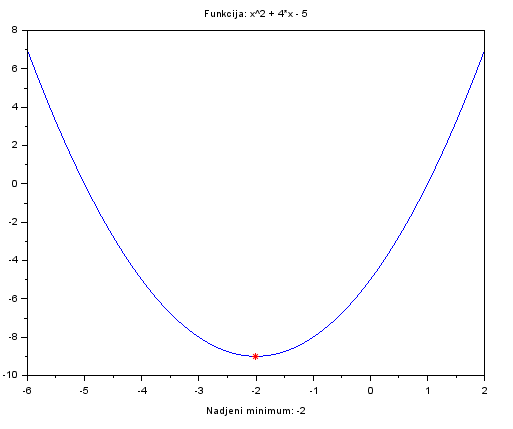
\includegraphics[scale=0.7]{parabola1.png}
\end{center}

\justify
Ukoliko uzmemo navedenu funkciju, samo prvi koeficijent pomnožimo sa -1, dobijemo funkciju $ y = -x^2 + 4x - 5 $ koja nema minimum, algoritam će proći kroz zadani broj \textit{maxiters} iteracija i ispisati poruku 'Minimum cannot be found within given number of iterations or it does not exist!'. 
\justify
Dalje, uzmimo funkciju $y = \frac{cos(3\pi\cdot x)}{x} $ koja ima beskonačno mnogo minimuma. Ukoliko kao početnu aproksimaciju uzmemo tačku $x = -1.1$ algoritam nakon 6 iteracija pronalazi minimum u tački -8.6653675, iako postoji minimum u tački -1.324854. Prikažimo ovo grafički:\\

\begin{center}
   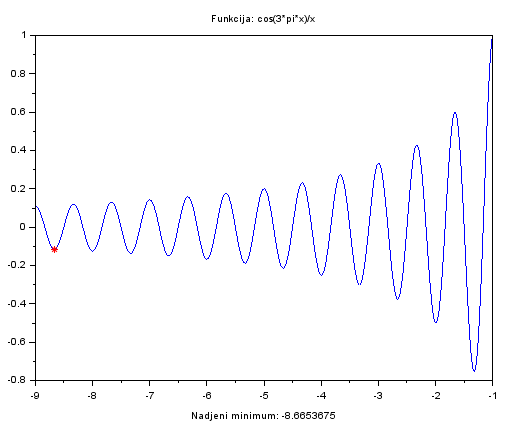
\includegraphics[scale=0.7]{cos.png}
\end{center}
\justify
Ovo je posljedica odabira jedinične matrice kao inicijalne vrijednosti Hessiana.



\subsection{Dvodimenzionalne funkcije}
\justify
Funkcije na koje ćemo se osvrnuti u ovom odjeljku su poznate funkcije korištene za testiranje algoritama za optimizaciju. I ovu skupinu funkcija započnimo sa najjednostavnijom između njih, odnosno \textbf{sfernom funkcijom} čija je formula 
$$ f(x, y) = x^2 + y^2 $$
i grafik:\\
\begin{center}
   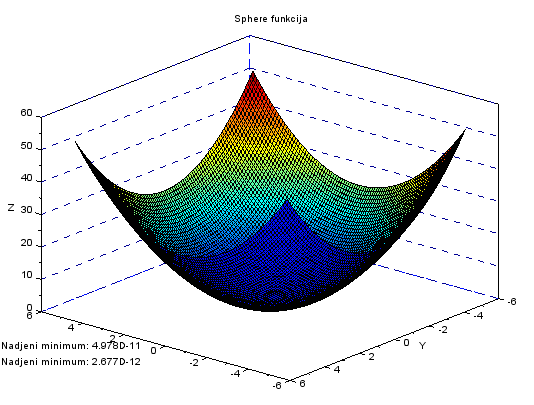
\includegraphics[scale=0.8]{spherefunction.png}
\end{center}

\justify
Vidimo da se globalni minimum ove funkcije nalazi u tački (0, 0), koju algoritam vrlo brzo pronalazi. Slično kao i za parabolu, BFGS daje tačan rezultat krenuvši iz ma koje tačke već u drugoj iteraciji.


\newpage
\justify
Testirajmo sada \textbf{Rosenbrockovu funkciju} koja predstavlja standardni test za testiranje algoritama za optimizaciju, a čija formula glasi:
$$ f(x, y) = b*(y - x^2)^2 + (a - x)^2, ~~ a,b\in\mathbb{R} $$
Naziva se još i banana funkcija zbog oblika nivo linija. Uzmemo li vrijednosti a=1 i b=100 njen grafik ima oblik:\\

\begin{center}
   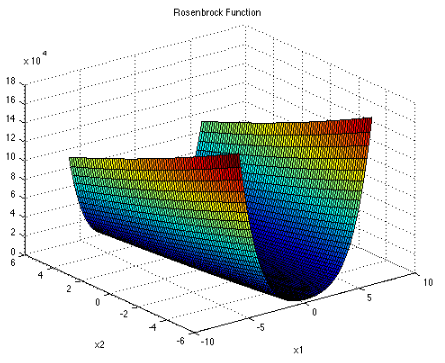
\includegraphics[scale=0.8]{rosenbrockfunction.png}
\end{center}

Kao što vidimo, njen globalni minimum (generalno tačka (a, a), konkretno (1, 1)) se nalazi u uskoj, paraboličnoj dolini koju je lako pronaći, ali konvergenciju prema minimumu je vrlo teško postići. Uzmimo nekoliko različitih tačaka i prikažimo broj iteracija do minimuma za svaku u sljedećoj tabeli:\\
\begin{center}
\begin{tabular}{|c|c|}
\hline
Tačka (x, y) & Broj iteracija \\ \hline
(2, 2)       & 42             \\ \hline
(-3, -3)     & 40             \\ \hline
(22, 54)     & 87             \\ \hline
(-72, 83)    & 101            \\ \hline
(8, -13)     & 38             \\ \hline
(110, 130)   & 105            \\ \hline
(112, 11)    & 67             \\ \hline
(544, 999)   & 202            \\ \hline
\end{tabular}
\end{center}


Još jedna poznata funkcija za testiranje ovih algoritama je \textbf{Rastriginova funkcija}. Za razliku od Rosenbrockove, ova funkcija ima veliki broj lokalnih i jedan globalni minimum u tački (0, 0). Njena formula glasi:
$$ f(x, y) = 20 + x^2 + y^2 -10*(cos(2\pi\cdot x) + cos(2\pi\cdot y)) $$
a grafik:\\

\begin{center}
   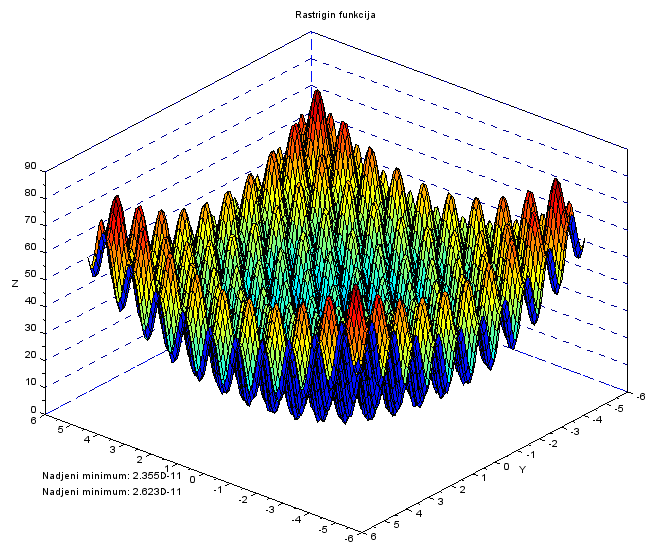
\includegraphics[scale=0.7]{rastriginfunction.png}
\end{center}

\justify
Iako ih ima mnogo, ovi minimumi su ravnomjerno raspoređeni i algoritam veoma brzo konvergira ka jednom, iako često dosta udaljenom od početne aproksimacije.\\


\justify
Prikažimo sada dvije dosta slične funkcije, Ackleyevu i Easomovu. Obje su neprekidne, nekonveksne i multimodalne. Formule im respektivno glase:

$$f(x, y) = -20e^{-0.2\sqrt{0.5(x^2 + y^2)}} - e^{0.5(cos(2\pi\cdot x) + cos(2\pi \cdot y ))} + 20 + e$$ 
$$f(x, y) = -cos(x)cos(y)e^{-(x-\pi)^2 - (y-\pi)^2}$$

\vspace*{0.5cm}

a grafici im respektivno imaju oblik:\\
\begin{minipage}{0.5\textwidth}
\begin{center}
   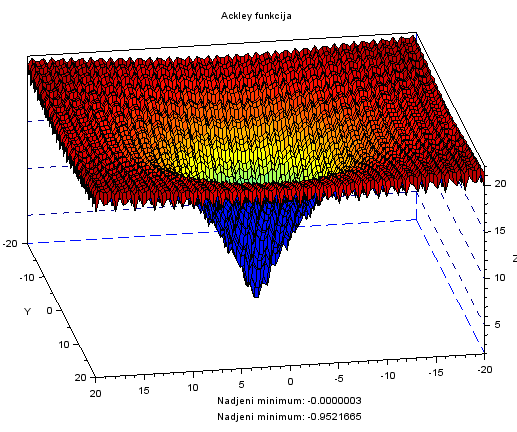
\includegraphics[scale=0.4]{ackleyfunction.png}
\end{center}
\end{minipage}
\begin{minipage}{0.5\textwidth}
\begin{center}
   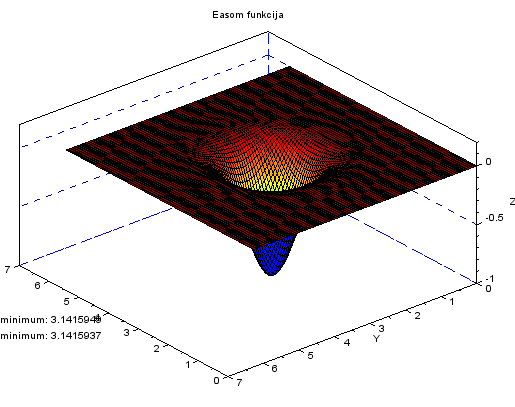
\includegraphics[scale=0.5]{easomfunction.png}
\end{center}
\end{minipage}

\justify
Globalni minimum Ackleyeve funkcije nalazi se u tački (0, 0), a Easomove u $(\pi, \pi)$. Pored ovoga, funkcije imaju veliki broj lokalnih minumuma koji predstavljaju veliki problem svim algoritmima za optimizaciju, pa i našem. Pored ovih minimuma, dio funkcija oko globalnog minimuma je prilično ravan, što dodatno otežava pretragu. Za obe ove funkcije algoritam se zaustavi u nekom od lokalnih minimuma blizu početne tačke, i to odmah u drugoj iteraciji, osim u slučaju kada se kao početna aproksimacija da tačka u blizini globalnog minimuma. U ovom slučaju, Wolfe-Powellovi uvjeti daju dobar korak koji često dovede do globalnog minimuma.\\


\justify
Prikažimo još neprekidnu, nekonveksnu i multimodalnu \textbf{Himmelblauevu funkciju} čija formula glasi:
$$ f(x, y) = (x^2 + y -11)^2 + (x + y^2 -7)^2 $$

\vspace*{1cm}

a grafik joj ima oblik:\\

\begin{center}
   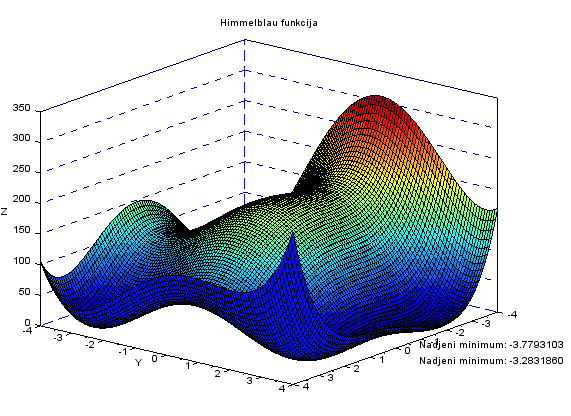
\includegraphics[scale=0.7]{himmelblaufunction.png}
\end{center}

\justify
Funkcija ima 4 globalna minimuma u tačkama (3, 2), (-2.8051181, 3.131312), (-3.779310, -3.283186) i (3.584428, -1.848126). Algoritam daje veoma dobre rezultate i dosta brzo konvergira ka nekom od ova 4 minimuma. Također, veoma je teško predvidjeti u kojem tačno minimumu će algoritam prekinuti izvršavanje, osim ako kao početnu aproksimaciju damo tačku dosta blizu jednom od njih.\\



\justify
U prilogu se nalaze rezultati testiranja još nekoliko sličnih funkcija, koje ovdje nećemo opisivati.






\subsection{Višedimenzionalne funkcije}
\justify
Većina prethodno spomenutih dvodimenzionalnih funkcija se može generalizirati u višedimenzionalni slučaj, za koje algoritam daje slične rezultate, proporcionalne s brojem promjenljivih. Kako smo ih već opisali, u ovom odjeljku razmotrimo drugu, karakterističnu funkciju za testiranje problema optimizacije.

\justify
Formula \textbf{Levyjeve funkciju} glasi:
$$ f(x) = sin^2(\pi w_i) + \sum_{i=1}^{d-1}(w_i-1)^2[1 + 10sin^2(\pi w_i +1)] + (w_d-1)^2[1+sin^2(2\pi w_d)] $$
gdje je d broj promjenljivih i
$$ w_i=1+\frac{x_i-1}{4}, ~~~ i=1, 2,...,d $$

\newpage
Kako ne možemo prikazati ovu funkciju u višedimenzionalnom slučaju, prikažimo njen grafik u slučaju dvije promjenljive:\\

\begin{center}
   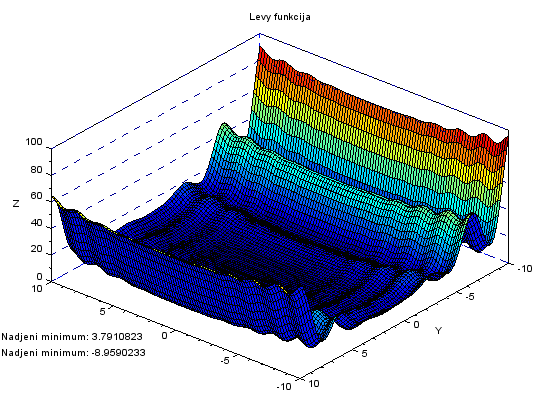
\includegraphics[scale=0.8]{levyfunction.png}
\end{center}


Ova funkcija ima globalni minimum u tački \textbf{x} = (1, 1, ..., 1), ali i dosta lokalnih minimuma zbog kojih algoritam teško završi u globalnom. 

\vspace*{0.75cm}

\justify
Još jedna poznata višedimenzionalna funkija za testiranje je \textbf{Hartmann-ova 6D funkcija}, koja ima 6 lokalnih minimuma, pri čemu je globalni

$$f(\textbf{x}^*) = -3.32237,$$ gdje je $$\textbf{x}^* = (0.20169, 0.150011, 0.476874, 0.275332, 0.311652, 0.6537)$$


\justify
Navedeni BFGS algoritam uspije naći globalni minimum u 30 iteracija za sljedeću početnu tačku:

$$\textbf{x}^* = (-1, 0.33, 0.8, -0.53, 0.22, 1)$$


\justify
Naravno, u ovisnosti od početne tačke broj iteracija može biti znatno manji odnosno veći.


\chapter{Primjene algoritma u praksi}


\justify
Generalno, problem minimizacije ima velike primjene u praksi. Investitori, proizvođači i inženjeri teže maksimalnoj efikasnosti u njihovom radu. Ovo postižu tako što odrede neki cilj koji može biti profit, vrijeme ili neka druga veličina. Dostizanje ovog cilja mora ovisiti o jednom ili nekoliko faktora, koje posmatramo kao varijable. Sve ovo se svodi na problem optimizacije n-dimenzionalne funkcije, s tim da se problem maksimizacije vrlo jednostavno svodi na minimizaciju.
\justify
Pored toga, ove probleme možemo primijetiti i u prirodnim procesima. Zakon o minimalnoj potencijalnoj energiji govori o tome da svaki sistem čestica, ili skupina istih, teži da zauzme takav položaj i raspored da njegova ukupna potencijalna energija bude minimalna.  Svjetlosne zrake putuju onim putem kojim stižu u minimalnom intervalu vremena. Molekule u izoliranom sistemu međusobno reaguju tako da im ukupna potencijalna energija bude minimalna. Ovakvih primjera ima još mnogo, sama priroda optimizira.
\justify
Konkretno, opisani algoritam rješava dosta navedenih problema, međutim, klasični Newtonov algoritam se vrlo rijetko koristi u praksi zbog svojih mnogih nedostataka. Jedan od glavnih razloga je taj što nemamo nikakvu garanciju da radimo sa silaznim pravcem, pa algoritam često terminira u nekom od lokalnih maksimuma, ili u nekoj sedlastoj tački. 
\justify
Razmotrimo naizled jednostavnu funkciju $y = x^3 + 3x^2 - 2x + 1$ koja ima jedan lokalni minimum u tački x = 0.2909944, te jedan lokalni maksimum u tački x = -2.2909944. Ukoliko funkciji \textit{Newton_Raphson} proslijedimo neku tačku iz intervala (-2.2909944, 0.2909944) algoritam nam kao rezultat u većini slučajeva vrati upravo lokalni maksimum. S druge strane, modificirani metod BFGS daje lokalni minimum. Prikažimo ovo grafički:\\



\begin{center}
   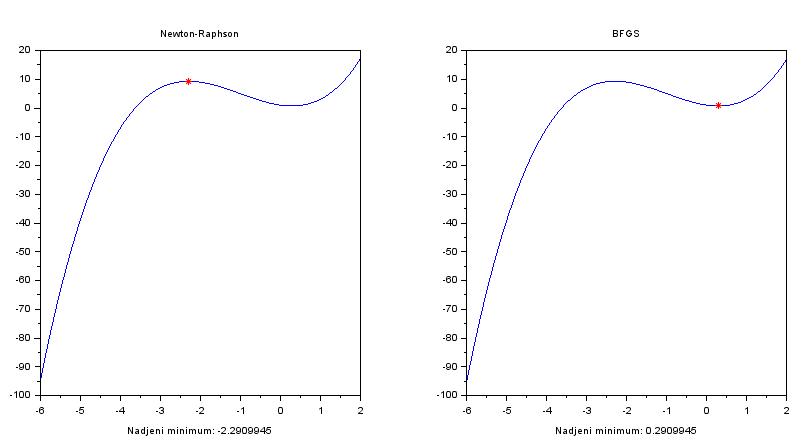
\includegraphics[scale=0.7]{nrvsbfgs.png}
\end{center}


Zanimljivo je spomenuti još neke probleme s ovom funkcijom. Naime, zbog naglog rasta, čak i metod BFGS za svaku vrijednost početne aproksimacije (x > 0.8) "preskoči" lokalni minimum i nastavi pretragu iza lokalnog maksimuma. Međutim, funkcija nakon ove vrijednosti samo opada, tako da algoritam terminira. Ovo je još jedan od razloga zbog kojeg se ovaj metod rijetko koristi sa jednodimenzionalnim funkcijama.
\justify
S druge strane, većina softverskih paketa za minimizaciju koristi upravo ovaj algoritam, ili se korisniku barem daje mogućnost njegovog  korištenja u slučaju da isti nije postavljen kao \textit{default} način. Konkretan primjer je programski paket korišten za implementaciju, Scilab, koji posjeduje predefinisani funkciju \textit{optim} u ovu svrhu. 
\justify
Vidjeli smo da i ovaj algoritam zakaže u nekim situacijama, pa postavljamo pitanje postoji li univerzalan algoritam koji daje optimalne rezultate. Odgovor je odričan. U praksi se često ne koristi konkretno jedan, nego optimizaciju vrši kombinacija većeg broja algoritama. Sve ovo ovisi o prirodi problema. Također, bitno je prepoznati ukoliko je došlo do greške, te iskorititi skupljeno znanje o problemu u svrhu poboljšanja rješenja. 


	\chapter{Zaključak i diskusija}
	Klasični Newton metod, njegove modifikacije kao i Quasi-Newton metode (BFGS specifično) predstavljaju veoma efikasan način pronalaska minimuma za funkcije više nezavisnih promjenljivih. Ne postoji generalno dobra strategija kada koji algoritam koristiti prilikom rješavanja problema optimizacije s obzirom da postoji širok spektar istih a ovdje su razmotreni samo metodi Newtonovog tipa. 
	
	\vspace{0.5cm}	
	\justify
	Uprkos tome pokazano je da su metodi ovog tipa veoma brzi i efikasni ukoliko se isti implementiraju na korektan način. 
	
	\vspace{0.5cm}
	\justify
	S obzirom da smo se bavili Newton-Raphson metodom i BFGS u nastavku navodimo potencijalne prednosti BFGS (u odnosu na klasični metod):
	
	\begin{itemize}
		\item potrebni su samo prvi izvodi (drugi)
		\item pozitivna definitnost Hessiana implicira silazni pravac (Hessian ne mora biti pozitivno definitan)
		\item Vremenska kompleksnost $O(n^2)$ ($O(n^3)$)
	\end{itemize}
	\justify
	
	
	\justify
	U algoritmima prezentiranim u ovom radu ostavljeno je dosta prostora za poboljšanje jer isti predstavljaju samo kostur za neku bolju i kompletniju implementaciju. Sam algoritam linijskog pretraživanja koji inkorporira sve nužne značajke za postizanje globalne konvergentnosti i bržeg terminiranja može biti poprilično težak zadatak. Za još bržu pretragu prikladnog koraka unutar intervala umjesto bisekcije preporučuje se i korištenje interpolacije drugog reda, eventualno trećeg. Također, može se desiti da, kako se približavamo rješenju, dvije uzastopne vrijednosti funkcija u dvije uzastopne iteracije mogu biti neprimjetne u aritmetici konačne preciznosti. Postoji još nekoliko stvari na koje treba obratiti pažnju za postizanje optimalnog rješenja. Jedna od najboljih implementacija algoritma linijskog pretraživanja je implementacija Moore-a i Thuente-a. Pogledati više na \cite{morethuente}.
	
	\justify
	Postavlja se i pitanje koliko je formula za ažuriranje Hessiana pouzdana, odnosno da li ista može uzrokovati loše rezultate. S obzirom da se radi o aritmetici konačne preciznosti jasno je da ne možemo očekivati perfekciju. Pa tako i algoritam prezentiran iznad posjeduje liniju koda koja terminira isti ukoliko se detektuje NaN vrijednost što se može desiti recimo ukoliko unutrašnji produkt $y_i s_i$ postane veoma mal ali pozitivan pri čemu će tada Hessian sadržavani ekstremno velike vrijednosti. U takvim slučajevima treba se voditi logikom \textit{"An ounce of prevention is better than a pound of cure"}. Također, performanse BFGS algoritma mogu poprilično degradirati ukoliko se linijska pretraga ne zasniva na Wolfe-Powell uvjetima. Za više informacija predlažemo \cite{nocedalwright}.
	
	\begin{thebibliography}{}
	\bibitem{nocedalwright}
	Jorge Nocedal, Stephen J. Wright:
	\textit{"Numerical Optimization", $2^{nd}$ edition,}
	Springer, New-York, 2006.
	
	\bibitem{zjuric}
	Željko Jurić:
	\textit{"Numerički algoritmi",}
	Elektrotehnički fakultet Univerziteta u Sarajevu, Sarajevo, 2018.
	
	
	\bibitem{morethuente}
	Jorge J. More and David J. Thuente:
	\textit{Line Search Algorithms with Guaranteed Sufficient Decrease,} ACM Transactions on Mathematical Software, Vol. 20, No. 3, September 1994.
	
	\bibitem{rfletcher}
	R.Fletcher:
	\textit{Practical Methods of Optimization,}
	University of Dundee, Scotland, UK, 1980.
	
	\bibitem{dennisschnabel}
	J.E. Dennis, Jr., Robert B. Schnabel:
	\textit{Numerical Methods for Unconstrained Optimization and Nonlinear Equations,}
	SIAM, 1996.
	
	\bibitem{robertfreud}
	Robert M. Freud:
	\textit{Newton’s Method for Unconstrained Optimization,}
	Massachusetts Institute of Technology, 2004.
\end{thebibliography}
\end{document}